\section{Analisi del contesto aziendale}
	\subsection{}
		\begin{frame}{L'azienda ospitante}
			\begin{figure}[H]
				\centering
				
\includegraphics[width=0.4\textwidth]{capitolo_1/immagini/logo_pastbook.png}
			\end{figure}
			\begin{figure}[H]
				\centering
				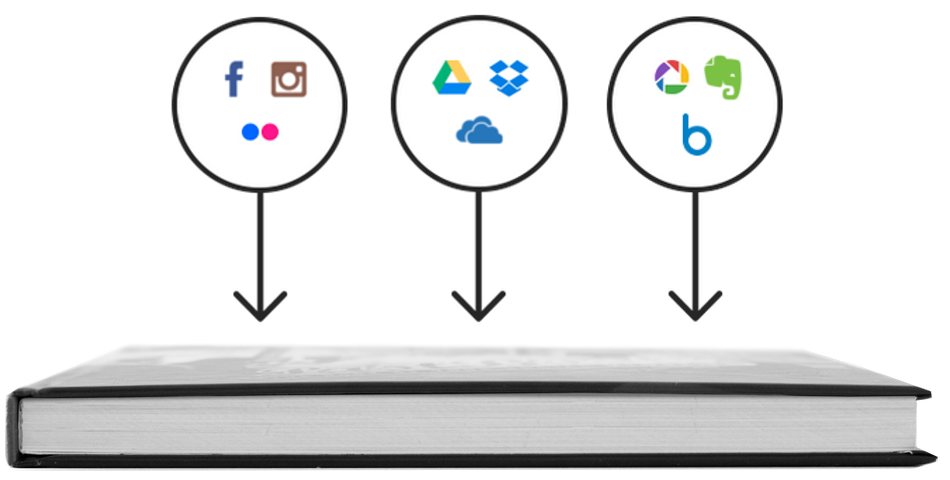
\includegraphics[width=0.9\textwidth]{capitolo_1/immagini/photo_book_one_click.png}
			\end{figure}
		\end{frame}
	\subsection{}
		\begin{frame}{Semplicità degli strumenti}
			\begin{itemize}
				\item \emph{Photo Book} in un click
				\item Il risultato deve piacere, non essere perfetto
				\item Personalizzazioni opzionali e basilari
			\end{itemize}
			\begin{figure}[H]
	\centering
	\begin{tikzpicture}
		\draw[fill=azzurro] (0,0) rectangle ++(0.26\textwidth,0.12\textwidth);
		\draw (0,0) rectangle ++(0.26\textwidth,0.12\textwidth)
		node[pos=.5, text width=0.24\textwidth, align=center] {Conquista utenti curiosi};
		\draw[fill=azzurro] (0.60\textwidth,0) rectangle ++(0.26\textwidth,0.12\textwidth);
		\draw (0.60\textwidth,0) rectangle ++(0.26\textwidth,0.12\textwidth)
		node[pos=.5, text width=0.24\textwidth, align=center] {Acquisti meno razionali};
		\draw[fill=azzurro] (0.30\textwidth,0.22\textwidth) rectangle ++(0.26\textwidth,0.12\textwidth);
		\draw (0.30\textwidth,0.22\textwidth) rectangle ++(0.26\textwidth,0.12\textwidth)
		node[pos=.5, text width=0.24\textwidth, align=center] {Semplicità degli strumenti};
		\draw[->] (0.40\textwidth,0.21\textwidth) -- (0.13\textwidth,0.13\textwidth);
		\draw[->] (0.46\textwidth,0.21\textwidth) -- (0.73\textwidth,0.13\textwidth);
	\end{tikzpicture}
\end{figure}

		\end{frame}
